131. \begin{figure}[ht!]
\center{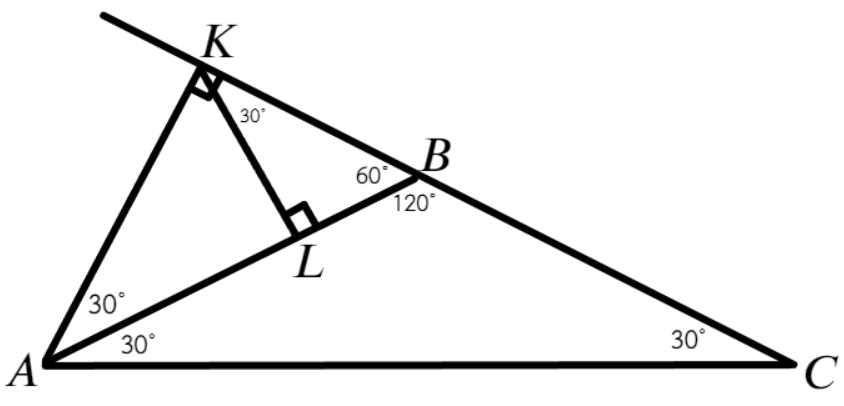
\includegraphics[scale=0.35]{g7-131.png}}
\end{figure}\\
Найдём $\angle KBL=180^\circ-120^\circ=60^\circ,\ \angle KAB=\angle LKB=90^\circ-60^\circ=30^\circ.$ Так как треугольник $ABC$ равнобедренный, $AB=BC=8$см. По теореме о катете, лежащем напротив угла в $30^\circ,$ получим $BK=\cfrac{1}{2}AB=\cfrac{1}{2}\cdot8=4,\ BL=\cfrac{1}{2}BK=\cfrac{1}{2}\cdot4=2$см.
ewpage
oindent
